% HiMCM 2026 Problem A manuscript.
% Provisional template control number; actual registration unverified. Shared class unchanged.
\documentclass{mcmthesis}
\mcmsetup{CTeX=false,tcn=18213,problem=A,sheet=true,titleinsheet=true,
keywordsinsheet=true,titlepage=false,abstract=true}
\usepackage{palatino,microtype,ragged2e,placeins,url,xurl}
\setlength{\headheight}{16pt}\urlstyle{same}\emergencystretch=3em\hyphenpenalty=500
\AtBeginDocument{\setlength{\parindent}{0pt}\setlength{\parskip}{0.5\baselineskip}}
\setlength{\tabcolsep}{5pt}
\widowpenalty=10000\clubpenalty=10000
\setcounter{tocdepth}{2}
\makeatletter
\renewcommand\tableofcontents{%
\centerline{\rmfamily\Large\bfseries\contentsname%
\@mkboth{\MakeUppercase\contentsname}{\MakeUppercase\contentsname}}%
\vskip 3ex\@starttoc{toc}}
\renewcommand{\l@section}{\def\@pnumwidth{2.3em}\def\@tocrmarg{2.3em}%
\bfseries\@dottedtocline{1}{1.5em}{2.3em}}
\renewcommand{\l@subsection}{\normalfont\@dottedtocline{2}{3.0em}{3.2em}}
\renewcommand{\@dotsep}{1}
\makeatother
\title{Choosing a City for High-School Life with Incomplete Evidence}
\author{}\date{}
\hypersetup{pdftitle={Choosing a City for High-School Life with Incomplete Evidence},pdfauthor={}}
\graphicspath{{./}{figures/}}

\begin{document}
\begin{abstract}
Among these sixteen cities, Zurich scores highest under priorities a high schooler would set,
with 64.5 points, a 1.2-point lead over Madrid; Singapore follows at 62.5.
Zurich stays first in all 31 source-variant checks of counting rules and source choices for transit stops, pools and travel. In broader withdrawals, Madrid leads when 64 entries dated after 2025 are treated as unknown, and Milan when 28 flagged entries or their 95-entry union with the dated groups are unknown. Zurich also leads in
82.8\% of 10,000 weight trials (concentration 100) and has the
smallest maximum regret, 6.1 points: the most it could trail the best rival
when every uncertain input breaks against it. The homicide input matters:
withdrawing Zurich's homicide value (treating it as unknown, utility range $[0,1]$) makes Madrid first.

We compare ten everyday measures using the analytic hierarchy process (AHP)
to assign weights. Each measure becomes a utility, a score from 0 to 1.
Safety and education each receive 34\% of the category weight. The
representative score is TOPSIS computed with the midpoint of each cell's utility range. Of 160 entries, 123 are single values, including
proxies, and 37 are utility ranges. Nine cities could lead under favorable
endpoints. Zurich remains first when education or mobility weights are doubled
separately, and the three hypothetical 2035 scenarios keep the top three unchanged.

\begin{keywords}
high-school city choice; AHP; TOPSIS; interval evidence; maximum regret; student priorities.
\end{keywords}
\end{abstract}
\maketitle
\clearpage
\tableofcontents

\clearpage
\section{Introduction and decision scope}
\subsection{What makes a city suitable for high-school life?}
A good city supports a student's school day through safety, affordable living,
teaching resources and convenient travel. We compare sixteen cities, one per
country, on ten everyday measures. Zurich leads Madrid by 1.2 points under our
high-schooler priorities. Section~\ref{sec:sourcepolicy} tests how source choices,
uncertain inputs and different priorities affect that recommendation.

A utility puts each measure on a scale from 0 to 1, with higher values better.
The \textbf{representative score} is TOPSIS computed with the midpoint of each
cell's utility range.

\subsection{Criterion selection and contribution}
Our criteria cover safety, air quality, housing and living costs, teaching
resources, higher education, transport stops, journey time, broadband and
swimming facilities (Table~\ref{tab:indicators}). Friendships, language and cultural
fit depend on the student; comparable surveys of wellbeing and discrimination
were unavailable. City totals also omit fees, eligibility and neighbourhood
routes. Families should check these factors against their needs and budget.

AHP gives pupils per teacher more weight than pools, reflecting their importance
to daily schooling. Compared with equal weights, twelve cities change rank;
Zurich remains first. The appended AI-use report describes assistance with
research, calculations and writing \cite{openai,exa}.

\section{Assumptions and their role}
\begin{enumerate}
\item \textbf{Source scopes stay fixed.} Mixed-year values retain their boundaries,
populations and school stages, so comparisons describe those source periods.
\item \textbf{Utilities use fixed scales.} More resources and lower burdens improve
utility; reference levels set the scales.
\item \textbf{Weights express our student priorities.} Safety and education each
receive 0.340, cost and mobility 0.123 each, and daily life 0.073, without a survey.
\item \textbf{Strengths can offset weaknesses.} Families should apply essential
safety or eligibility thresholds before using the combined score.
\item \textbf{Utility ranges vary independently.} Endpoint tests of the 37 utility
ranges assume independent variation; possible winners and maximum regret depend on it.
\item \textbf{Scenarios hold the comparison basis fixed.} Population denominators,
reference levels and weights stay unchanged.
\end{enumerate}

\section{Notation}
\begin{tabular}{p{.18\linewidth}p{.75\linewidth}}
\toprule Symbol & Meaning\\\midrule
$x,a$ & Observed indicator value and reference level (in the same units)\\
$u,u_{ij}$ & Utility on $[0,1]$; $i$ identifies a city and $j$ an indicator\\
$c,P,d$ & Count, population and density (institutions per million; stops and pools per 100,000)\\
$t,q$ & Travel duration in minutes and its utility\\
$w_j$ & Indicator weight, with all ten weights summing to one\\
$D_i^+,D_i^-$ & City $i$'s distances to the ideal and worst utility profiles\\
$S_i$ & City $i$'s TOPSIS score, on $[0,100]$\\
$\ell_{ij},h_{ij}$ & Lower and upper utility bounds\\
$L_i,U_i$ & Lower and upper score bounds, $S(\ell_i)$ and $S(h_i)$\\
$R_i$ & Maximum regret\\
$\kappa$ & Concentration of a declared Dirichlet weight distribution\\
$r$ & Raw-value multiplier in a development scenario\\\bottomrule
\end{tabular}

\section{Indicator construction and city selection}
\FloatBarrier
\subsection{City selection}\label{sec:citychoice}
The sixteen cities are Amsterdam, Berlin, Dublin, Helsinki, London, Madrid,
Milan, Oslo, Paris, Prague, Singapore, Stockholm, Tokyo, Vienna, Warsaw and
Zurich. The primary comparison uses one city from each of sixteen countries.
The set spans cost, climate, population scale, mobility and safety
(Table~\ref{tab:cityset}). Fourteen cities are European and all are in high-income
economies; the recommendation applies to these sixteen candidates.

The locations and final ranks are shown in Figure~\ref{fig:citymap}.
\begin{figure}[!htbp]\centering
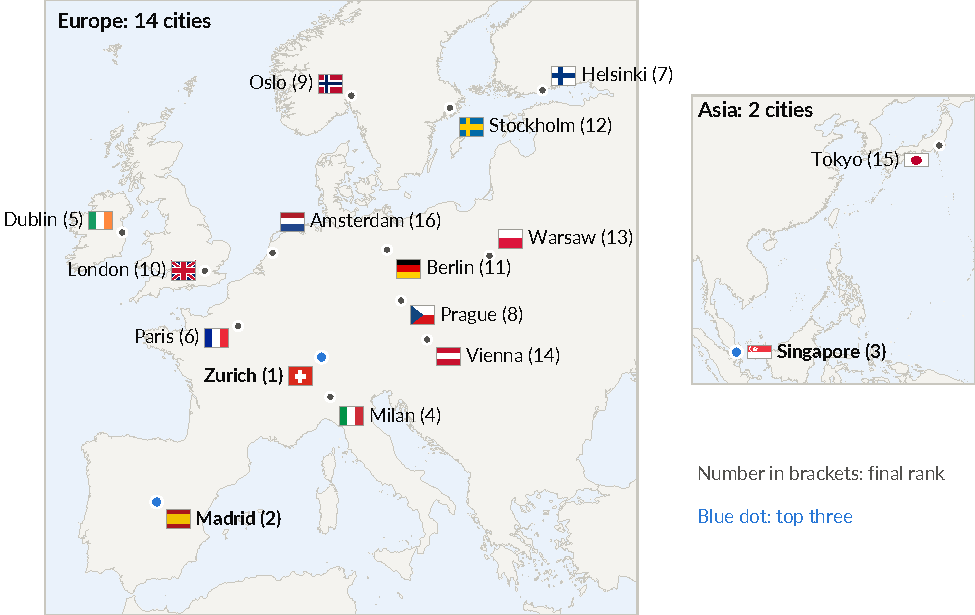
\includegraphics[width=\linewidth]{figures/city_map.pdf}
\caption{The 16 candidate cities, with national flags and final ranks in brackets; blue dots mark the top three.}\label{fig:citymap}
\end{figure}

One city per country avoids repeating national data systems and school
structures. City records take priority; national statistics or surveys provide
the labelled proxies listed in Section~4.3. Table~\ref{tab:cityprofile} counts the
evidence labels; some team-table values lack original links and are tested by
withdrawal in Section~\ref{sec:sourcepolicy}.

\begin{table}[!htbp]\centering
\caption{City profiles and evidence labels. Direct values are official or team-table values; ranges and proxies are counted separately.}\label{tab:cityprofile}
\begingroup\scriptsize\setlength{\tabcolsep}{3pt}
\begin{tabular}{@{}l l r r r r@{}}
\toprule City & Country & Population (year) & Direct values & Utility ranges & Proxies\\\midrule
Vienna & Austria & 2,028,399 (2025) & 8 & 1 & 1\\
Zurich & Switzerland & 440,935 (2025) & 6 & 3 & 1\\
Helsinki & Finland & 694,392 (2025) & 7 & 2 & 1\\
Berlin & Germany & 3,700,577 (2025) & 8 & 2 & 0\\
London & United Kingdom & 9,122,909 (2025) & 7 & 2 & 1\\
Amsterdam & Netherlands & 941,927 (2025) & 7 & 2 & 1\\
Stockholm & Sweden & 999,200 (2025) & 6 & 4 & 0\\
Paris & France & 2,103,778 (2023) & 7 & 2 & 1\\
Madrid & Spain & 3,527,924 (2025) & 7 & 2 & 1\\
Milan & Italy & 1,399,079 (2025) & 6 & 3 & 1\\
Dublin & Ireland & 592,713 (2022) & 7 & 2 & 1\\
Oslo & Norway & 727,797 (2025) & 8 & 2 & 0\\
Prague & Czechia & 1,407,084 (2025) & 7 & 3 & 0\\
Warsaw & Poland & 1,863,800 (2024) & 7 & 2 & 1\\
Singapore & Singapore & 6,036,900 (2024) & 7 & 3 & 0\\
Tokyo & Japan & 9,983,365 (2026) & 7 & 2 & 1\\
\midrule Total &  &  & 112 & 37 & 11\\
\bottomrule\end{tabular}\endgroup
\par\vspace{8pt}
\caption{The sixteen cities distribute across the dimensions the indicators measure.}\label{tab:cityset}
\begin{tabular}{@{}p{.28\linewidth}p{.68\linewidth}@{}}
\toprule Dimension & Span within the set\\\midrule
Cost of living & Moderate capitals (Warsaw, Prague, Madrid, Berlin) to among the world's most expensive (Zurich, Oslo, London, Singapore)\\
Climate & Cold northern (Oslo, Helsinki, Stockholm) and continental (Berlin, Vienna, Warsaw, Prague) through maritime (London, Dublin, Amsterdam) and warm Mediterranean (Madrid, Milan) to tropical Singapore and humid-subtropical Tokyo\\
Scale & Mid-size capitals (Zurich, Oslo, Helsinki, Dublin) up to large metropolises (Tokyo, London, Paris)\\
Mobility & Cycling and tram networks (Amsterdam, Berlin, Prague, Vienna) to dense metro systems (Tokyo, Paris, London)\\
Safety & Low recorded homicide rates (Singapore, Tokyo, Oslo) alongside higher rates elsewhere in the set\\
\bottomrule
\end{tabular}
\end{table}

\FloatBarrier
\subsection{Indicator system}\label{sec:indicators}
The ten indicators form five categories, with two indicators in each category.
Table~\ref{tab:indicators} gives the unit, direction, anchor and data note in
one place. Utilities lie on $[0,1]$, with larger values always preferred.

\begin{table}[!htbp]\centering
\caption{Indicator definitions, anchors and data treatment.}\label{tab:indicators}
\begingroup\footnotesize\setlength{\tabcolsep}{2.8pt}
\begin{tabular}{@{}>{\raggedright\arraybackslash}p{.15\linewidth}>{\raggedright\arraybackslash}p{.22\linewidth}>{\raggedright\arraybackslash}p{.12\linewidth}>{\raggedright\arraybackslash}p{.10\linewidth}>{\raggedright\arraybackslash}p{.14\linewidth}>{\raggedright\arraybackslash}p{.21\linewidth}@{}}
\toprule Category & Indicator & Unit & Better when & Anchor $a$ & Data note\\\midrule
Safety and environment & Homicide rate & Deaths per 100,000 & Lower & 2 deaths per 100,000 & City record; Zurich recalculated\\
 & PM$_{2.5}$ concentration & $\mu$g/m$^3$ & Lower & 15 $\mu$g/m$^3$ & City record\\\midrule
Cost of living & Living-cost index & Index points & Lower & 100 points & City record\\
 & Housing price-to-income ratio & Ratio & Lower & 10 & City record\\\midrule
Education & Upper-secondary pupils per teacher & Pupils per teacher FTE & Lower & 15 pupils/FTE & City record; proxy fills\\
 & Higher-education institutions & Institutions per million & Higher & 10 per million & City record\\\midrule
Mobility & Mean travel/commute time & Minutes & Lower & 30-minute decay scale & City record; survey proxies and utility ranges\\
 & Public-transport stops & Stops per 100,000 & Higher & 50 per 100,000 & City record; utility ranges for uncounted providers\\\midrule
Daily life & Fixed broadband speed & Mbps & Higher & 100 Mbps & City record\\
 & Public swimming pools & Venues per 100,000 & Higher & 1 per 100,000 & City record; utility ranges for uncounted providers\\
\bottomrule
\end{tabular}\endgroup
\end{table}

For a benefit and cost indicator, respectively, utility is
\begin{equation}
 u=\frac{x}{a+x},
 \label{eq:benefit}
\end{equation}
and
\begin{equation}
 u=\frac{a}{a+x}.
 \label{eq:cost}
\end{equation}
The anchor $a$ gives utility 0.5 when $x=a$. Higher-education density is
$10^6c/P$ institutions per million, with anchor 10 per million.

For transport stops and pools, facility counts become density per 100,000:
\begin{equation}
 d=\frac{100000c}{P}.
 \label{eq:density}
\end{equation}
We use $x=d$ in Equation~\ref{eq:benefit}; a verified subset gives the lower
utility bound and the upper bound remains 1 when other providers are uncounted.

Upper-secondary teaching resources use pupils per full-time-equivalent (FTE)
teacher:
\begin{equation}
 x=\frac{\text{upper-secondary pupils}}{\text{upper-secondary teacher FTE}}.
 \label{eq:ptr}
\end{equation}
Prague's 2024/25 records give about 11.6 pupils per teacher after lower-gymnasium
years are removed \cite{prague}.

For travel, a journey of $t$ minutes has utility
\begin{equation}
 q=\exp(-t/30).
 \label{eq:travel}
\end{equation}
When only a mean duration $\bar t$ is available, its utility range is
\begin{equation}
 \mathbb{E}[q]\in[\exp(-\bar t/30),1].
 \label{eq:travel-range}
\end{equation}
The lower endpoint follows from convexity, and 1 is the upper limit for
nonnegative durations. Work-commute means describe general travel conditions;
Singapore's school-stage bins provide a separate range \cite{eurostatcommute,singapore}.

Figure~\ref{fig:indicator-compare} compares the cities on the shared utility
scale. Singapore and Milan have the highest homicide utilities (0.97 and 0.89),
while Amsterdam has 0.06; Madrid has the lowest pupil-teacher proxy ratio at 9.6
pupils per teacher and utility 0.61.

Figure~\ref{fig:raw} shows the raw values, including Zurich's higher-education
supply of 52 institutions per million.

\begin{figure}[!htbp]\centering
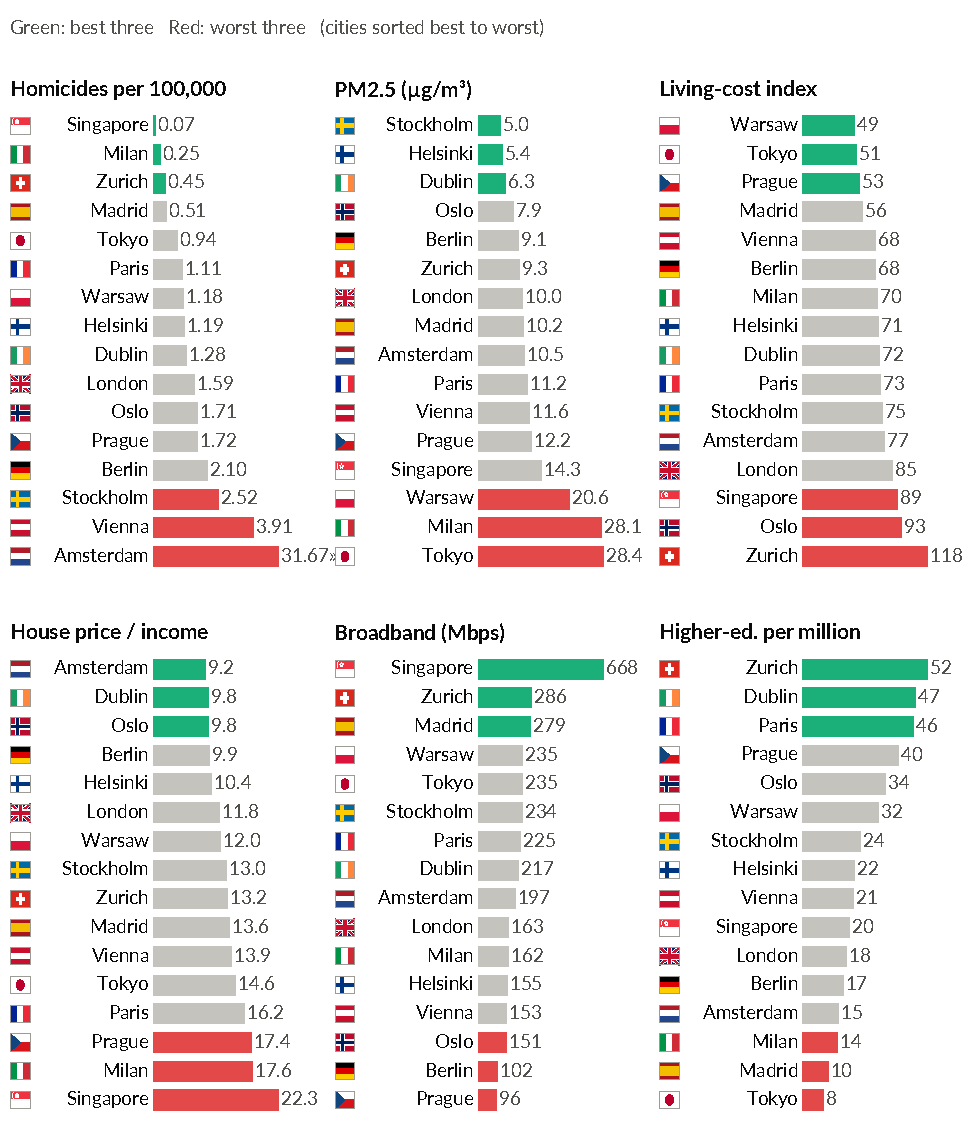
\includegraphics[width=\linewidth]{figures/raw_compare.pdf}
\caption{Raw values for the six indicators with complete city records, ordered from best to worst within each indicator. The best three cities are green and the worst three red; flags identify countries. Homicides are shown per 100,000, with Zurich's recalculated 0.45 and Amsterdam's 31.67 marked off-scale with ``$\gg$''. Higher-education supply is institutions per million.}\label{fig:raw}
\end{figure}

\begin{figure}[!htbp]\centering
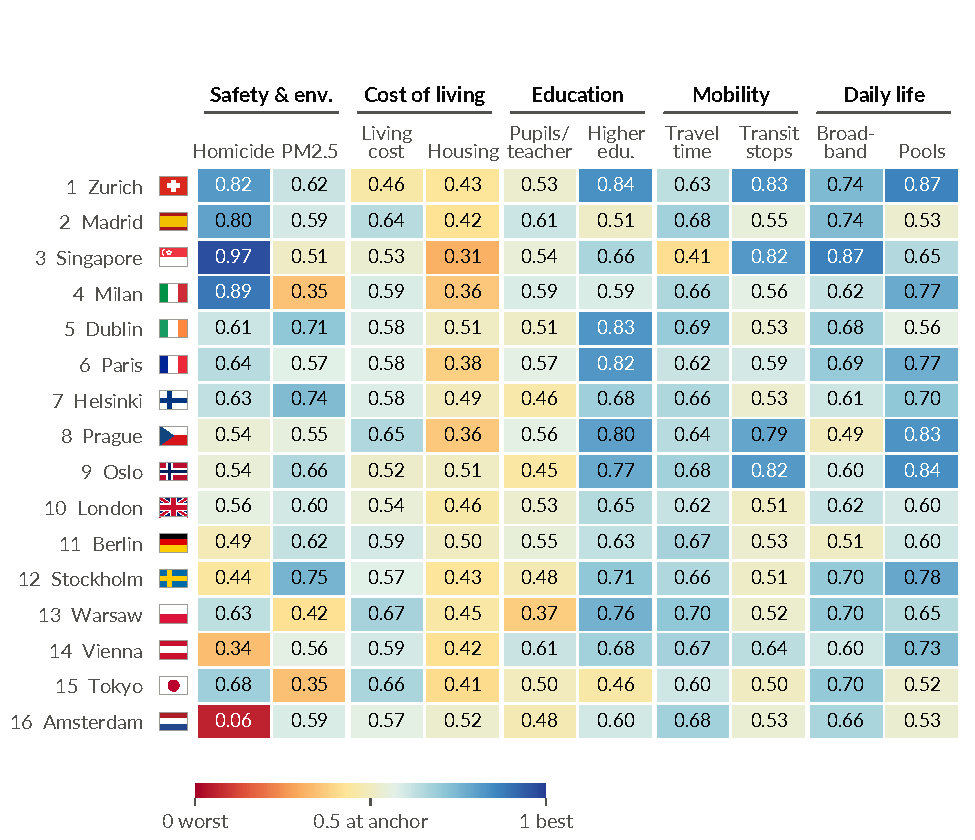
\includegraphics[width=\linewidth]{figures/indicator_compare.pdf}
\caption{Indicator utilities for the sixteen cities, ordered by final score and grouped by category. Colour is utility from 0 (worst) to 1 (best). Utility ranges show their midpoint with a black corner triangle, proxies have a dashed outline, and flags mark countries.}\label{fig:indicator-compare}
\end{figure}

\FloatBarrier
\subsection{Data sources and filled values}
The team table supplies the base matrix and its source years and boundaries
\cite{teamtable}. Table~\ref{tab:sources} lists the principal source families.

Three construction rules keep measurements comparable:
\begin{enumerate}
\item Count each station once, excluding separate platforms and repeated line
entries. Warsaw's 21 M1 and 18 M2 entries give 38 stations after merging the
shared \'Swi\k{e}tokrzyska interchange \cite{warsawmetro}.
\item Match school stage before dividing pupils by teacher FTE. Prague's totals
therefore remove lower-gymnasium pupils and teachers \cite{prague}.
\item Recalculate Zurich's supplied 0.14 as 0.45 per 100,000: two completed
homicide offences recorded by the Zurich city police in 2025, divided by
440,935 residents \cite{zhpks2025}. A rate built on two events is unstable.
\end{enumerate}
Tokyo's Oedo directory contributes 38 distinct stations in the 23 wards, and
Oslo's inventory uses parent stop groups; the questioned Tveten bru entry is
excluded because its closure is unconfirmed \cite{tokyooedo,enturstop}.

The 11 proxy cells are six Eurostat national pupil-teacher ratios from table
educ\_\allowbreak uoe\_\allowbreak perp04 (ISCED 3, 2024), two median pupil-teacher values of 13.45 for
Zurich and London, and three survey travel means entering as utility ranges:
Vienna 32 minutes, Tokyo 47.5 minutes from the 2021 Japanese time-use survey,
and Warsaw 27 minutes \cite{warsaw2022}. The Eurostat ratios are Helsinki 17.4,
Amsterdam 16.4, Dublin 14.2, Paris 11.5, Milan 10.6 and Madrid 9.6.

The 160 entries comprise 123 single values, including proxies, and 37 utility
ranges. Zurich's homicide recalculation is separate from the 11 proxies.

\begin{table}[!htbp]\centering
\caption{Sources and years by indicator. Supplements establish counted subsets, proxies and boundary rules for the team matrix.}\label{tab:sources}
\begingroup\small\setlength{\tabcolsep}{3pt}
\begin{tabular}{@{}p{.18\linewidth}p{.34\linewidth}p{.12\linewidth}p{.29\linewidth}@{}}
\toprule Indicator & Main sources & Year(s) & Notes \\\midrule
Homicide rate & Team table; Zurich police statistics \cite{teamtable,zhpks2025}; CBS recount for Amsterdam \cite{cbshomicide2022} & 2022--2025 & Zurich: two completed offences recorded by city police in 2025; 440,935 residents; rate 0.45 per 100,000. \\
PM$_{2.5}$ & Team table & 2021--2025 & City monitoring values with reported station and year scopes. \\
Living-cost index & Team table \cite{teamtable} & 2025--2026 & City index values; source year stays attached to each row. \\
Housing price-to-income & Team table; Oslo property-price archive \cite{teamtable,numbeooslo2026} & 2025--2026 & City price-to-income values; administrative boundaries follow the team matrix. \\
Upper-secondary pupils per teacher & Team table; Prague, Paris, Finland and Ireland education records; Eurostat proxy fills \cite{teamtable,prague,parisedu,finlandfte,irelandfte,irelandpayroll,warsawedu2025,kolada,shanghai,sgage} & 2024--2026 & Six Eurostat national ratios and two median fills for Zurich and London are labelled proxies; Prague is stage-matched; Shanghai and Singapore stage tables support supplementary records. \\
Higher-education institutions & Team table; school and post-secondary directories \cite{teamtable,deppmatch,deppdirectory} & 2025--2026 & Institutions per million; each provider counted once, with cross-stage providers flagged. \\
Mean travel/commute time & Team table; Eurostat city series; Warsaw school-trip survey; Singapore census bins \cite{teamtable,eurostatcommute,warsaw2022,singapore,dublin} & 2011--2024 & Vienna, Tokyo and Warsaw means enter as utility ranges; work-commute means are proxies for general travel conditions. \\
Public-transport stops & Operator and municipal inventories for Oslo, Zurich, Helsinki, Madrid, Vienna, Prague, Berlin, London, Singapore, Amsterdam, Milan, Stockholm, Tokyo and Warsaw \cite{oslo,enturstop,vbz,helsinki,madridmetro,viennaogd,viennagis,pidmetro,dpp2025,floraclose,bvg,tflinventory,sgbus_lta,amsterdammetro2026,milanmetro,stockholmmetro2025,tokyooedo,warsawmetro,warsawfirescope,inecodes,onslondon,cbsboundary2025} & 2024--2026 & Operator inventories, counted once per station; interchange and boundary rules are explicit, with verified subsets forming lower bounds. \\
Fixed broadband speed & Team table & 2025--2026 & City speed observations with the reported test window. \\
Public swimming pools & Team table; municipal and operator inventories for Stockholm, Paris, Tokyo, Singapore, Zurich and Milan \cite{teamtable,stockpool,apur,nerimapool,nerimaclose,sgpool_directory,sgocbc,sgpool_2025,zurichpool,milanpool2025} & 2025--2026 & Venues counted once per provider; operator inventories are lower bounds when coverage is incomplete. \\
\bottomrule
\end{tabular}\endgroup
\end{table}


\FloatBarrier
\section{Establishing the baseline evaluation model}
\FloatBarrier
\subsection{Determining indicator weights (AHP)}
\textbf{Step 1: Set up the hierarchy.}
We use the analytic hierarchy process (AHP) to turn our student priorities
into weights: the goal is city choice, followed by five categories and their
ten indicators \cite{saaty}.

\textbf{Step 2: Compare the five categories.}
Table~\ref{tab:ahp-categories} uses Saaty's 1--9 importance scale, with 1 for
equal importance and reciprocal entries for reverse comparisons.
Safety and schooling come first; cost and mobility support the family budget
and daily journeys, while broadband and pools receive less weight.

\begin{table}[!htbp]\centering
\caption{Pairwise category comparisons from our student viewpoint. S: safety and
environment; C: cost of living; E: education; M: mobility; D: daily life.}\label{tab:ahp-categories}
\begin{tabular}{lccccc}
\toprule Category & S & C & E & M & D\\\midrule
Safety and environment & 1 & 3 & 1 & 3 & 4\\
Cost of living & $1/3$ & 1 & $1/3$ & 1 & 2\\
Education & 1 & 3 & 1 & 3 & 4\\
Mobility & $1/3$ & 1 & $1/3$ & 1 & 2\\
Daily life & $1/4$ & $1/2$ & $1/4$ & $1/2$ & 1\\
\bottomrule
\end{tabular}
\end{table}

\textbf{Step 3: Calculate category weights and check consistency.}
For comparison matrix $A$, find its largest eigenvalue $\lambda_{\max}$ and
positive eigenvector $v$, then normalise $v$ to sum to one for category weights $g_k$:
\begin{equation}
 Av=\lambda_{\max}v.
 \label{eq:ahp-eigenvector}
\end{equation}
With five categories ($n=5$), the consistency index and consistency ratio are
\begin{equation}
 CI=\frac{\lambda_{\max}-n}{n-1}.
 \label{eq:ahp-ci}
\end{equation}
\begin{equation}
 CR=\frac{CI}{RI}.
 \label{eq:ahp-cr}
\end{equation}
The random index is $RI=1.12$; our matrix gives $\lambda_{\max}=5.0264$,
$CI=0.00660$ and $CR=0.0059<0.1$, meeting the consistency threshold \cite{saaty}.

\textbf{Step 4: Compare the two indicators within each category.}
Our local importance ratios are 2:1 for homicide to PM$_{2.5}$, 1:1 for living
costs to housing, 3:1 for teacher resources to higher-education supply, 2:1 for
travel time to stops, and 2:1 for broadband to pools. These choices emphasise
personal safety, current schooling, journey time and schoolwork; each pair
and its reciprocal give an internally consistent two-indicator matrix.
The local weight $p_j$ is its share of the pair's ratio, giving global weight
\begin{equation}
 w_j=g_k p_j.
 \label{eq:global-weights}
\end{equation}
Figure~\ref{tab:ahp-weights} shows both levels; calculations use unrounded weights.

\begin{figure}[!htbp]\centering
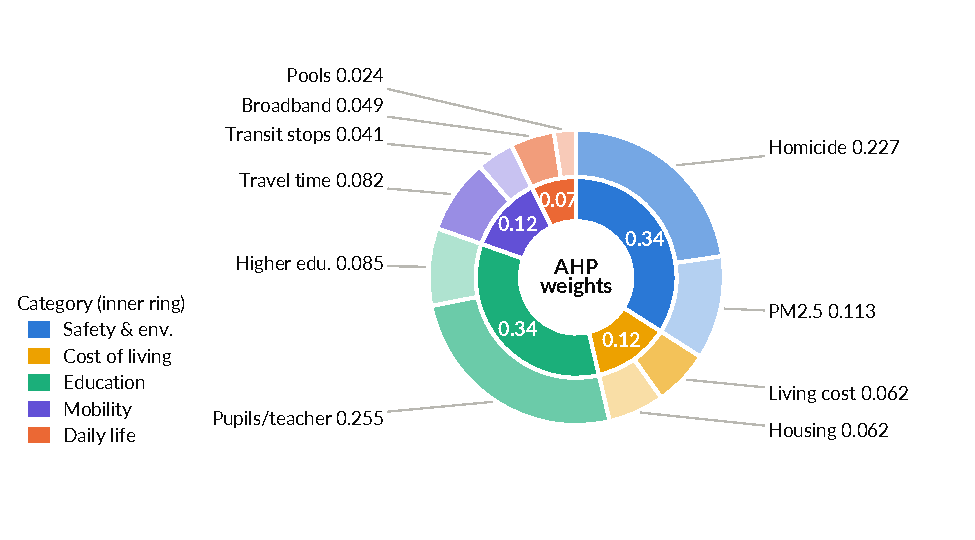
\includegraphics[width=\linewidth]{figures/ahp_weights.pdf}
\caption{AHP weights from our student priorities. The inner ring shows the five
category weights; the outer ring shows the ten global indicator weights,
printed beside each slice. Safety and environment and education each receive
0.340.}\label{tab:ahp-weights}
\end{figure}

\FloatBarrier
\subsection{TOPSIS scoring}
\textbf{Step 1: Form the utility matrix.}
For the representative score, using the arithmetic midpoint of each utility range $[\ell_{ij},h_{ij}]$ is a modelling choice on the shared 0--1 scale. Endpoint values are used only in the robustness checks:
\begin{equation}
 u_{ij}=\frac{\ell_{ij}+h_{ij}}{2}.
 \label{eq:representative-utility}
\end{equation}

\textbf{Step 2: Find the distance to the ideal.}
A smaller $D_i^+$ means fewer weighted shortfalls from the all-one ideal \cite{topsis}:
\begin{equation}
 D_i^+=\sqrt{\sum_{j=1}^{10}w_j(1-u_{ij})^2}.
 \label{eq:distance-ideal}
\end{equation}

\textbf{Step 3: Find the distance to the worst profile.}
A larger $D_i^-$ means stronger performance above the all-zero profile:
\begin{equation}
 D_i^-=\sqrt{\sum_{j=1}^{10}w_j u_{ij}^2}.
 \label{eq:distance-worst}
\end{equation}

\textbf{Step 4: Calculate the score.}
TOPSIS gives the representative score $S_i$ from 0 to 100, with higher values preferred:
\begin{equation}
 S_i=100\frac{D_i^-}{D_i^++D_i^-}.
 \label{eq:topsis-score}
\end{equation}

\textbf{Step 5: Carry utility ranges into the score.}
Since the score rises with every utility, the lower and upper utility vectors
$\ell_i$ and $h_i$ give the score bounds used in sensitivity checks:
\begin{equation}
 [L_i,U_i]=[S(\ell_i),S(h_i)].
 \label{eq:score-range}
\end{equation}

\FloatBarrier
\subsection{Scoring results and interpretation}
Zurich leads with a representative score of 64.5, followed by Madrid and
Singapore (Table~\ref{tab:baseline}). Figure~\ref{fig:radar} contrasts tiers using
representative cities: the whole top tier (ranks 1--3), the lower end of the
middle tier (7--9) and the lowest three cities (14--16).

\begin{table}[!htbp]\centering
\caption{Representative scores under AHP weights, using the midpoint of each utility range.}
\label{tab:baseline}
\begingroup\setlength{\tabcolsep}{3pt}
\begin{tabular}{rlrl@{\qquad}rlrl}\toprule
Rank & City & Score & Tier & Rank & City & Score & Tier\\\midrule
\textbf{1} & \textbf{Zurich} & \textbf{64.5} & \textbf{Top} & \textbf{9} & \textbf{Oslo} & 57.6 & Middle\\
\textbf{2} & \textbf{Madrid} & 63.3 & Top & \textbf{10} & \textbf{London} & 56.1 & Bottom\\
\textbf{3} & \textbf{Singapore} & 62.5 & Top & \textbf{11} & \textbf{Berlin} & 55.6 & Bottom\\
\textbf{4} & \textbf{Milan} & 61.1 & Middle & \textbf{12} & \textbf{Stockholm} & 55.4 & Bottom\\
\textbf{5} & \textbf{Dublin} & 60.8 & Middle & \textbf{13} & \textbf{Warsaw} & 54.5 & Bottom\\
\textbf{6} & \textbf{Paris} & 60.8 & Middle & \textbf{14} & \textbf{Vienna} & 54.4 & Bottom\\
\textbf{7} & \textbf{Helsinki} & 58.7 & Middle & \textbf{15} & \textbf{Tokyo} & 54.0 & Bottom\\
\textbf{8} & \textbf{Prague} & 58.4 & Middle & \textbf{16} & \textbf{Amsterdam} & 45.2 & Bottom\\
\bottomrule\end{tabular}\endgroup\end{table}

\textbf{Top tier.} Ranks 1--3, Zurich, Madrid and Singapore, score 62.5--64.5 through
strength in safety and environment and education, the two heaviest categories.
Zurich combines category scores of 0.75 and 0.61, Madrid 0.73 and 0.59,
and Singapore 0.81 and 0.57.

\textbf{Middle tier.} Ranks 4--9, Milan through Oslo, score 57.6--61.1, starting 1.4 points
below Singapore; a strong category is paired with a weaker one.
For example, Helsinki scores 0.66 for safety and environment and 0.52 for
education, while Prague scores 0.62 for education and 0.54 for safety and environment.

\textbf{Bottom tier.} Ranks 10--16, London through Amsterdam, score 45.2--56.1, starting
1.4 points below Oslo, as one or two heavily weighted utilities pull scores down.
Vienna's safety and environment score is 0.41 despite education at 0.63;
Amsterdam's homicide utility of 0.06 leaves it 8.8 points behind Tokyo.

\begin{figure}[!htbp]\centering
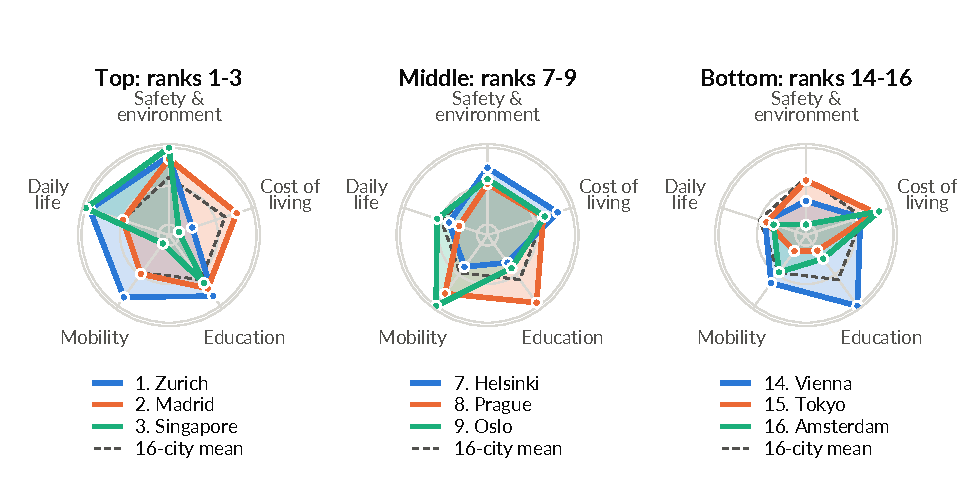
\includegraphics[width=\linewidth]{figures/radar_tiers.pdf}
\caption{Representative cities chosen to contrast tiers: the whole top tier
(ranks 1--3), the lower end of the middle tier (7--9), and the lowest three
cities (14--16). Each axis is
stretched from the lowest city (centre) to the highest city (outer ring) among
all sixteen; the dashed line is the sixteen-city mean. Category scores combine
each pair of indicators using its local AHP weights.}
\label{fig:radar}
\end{figure}

\FloatBarrier
\subsection{A significant revision: from equal weights to AHP weights}
Equal weights give every indicator 0.1, making pools as influential as homicide
or teacher resources. AHP expresses our student priorities: safety and environment
and education each receive 0.340, cost and mobility 0.123 each, and daily life 0.073.

With utilities, anchors and scoring unchanged, the leading four shift from
Zurich, Oslo, Paris and Dublin to Zurich, Madrid, Singapore and Milan.
Twelve of sixteen cities change rank, with Kendall's $\tau=0.517$ measuring
agreement between the two rankings. Zurich stays first; the revised top group
reflects the greater weight on safety and schooling.

\FloatBarrier
\subsection{Robustness of the recommendation}\label{sec:sourcepolicy}
\textbf{Score bounds and maximum regret.} Figure~\ref{fig:robust} carries the score intervals, representative scores and weight-draw frequencies. Maximum regret is the most a city could trail the best rival when every utility range breaks against it:
\begin{equation}
 R_i=\max\left\{0,\max_{k\ne i}U_k-L_i\right\}.
 \label{eq:regret}
\end{equation}
Zurich has the smallest maximum regret, 6.1 points; nine cities can be first under some endpoint combination.

\begin{figure}[!htbp]\centering
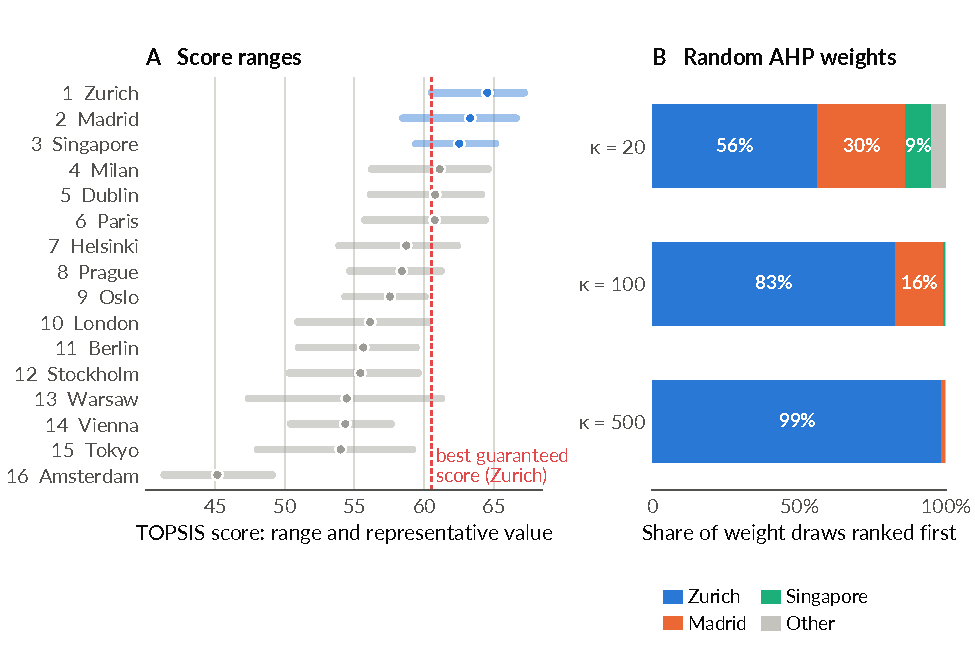
\includegraphics[width=\linewidth]{figures/robustness.pdf}
\caption{Robustness of the recommendation. Panel A shows each city's score interval as a light bar and its representative score as a dot; the top three are blue and the dashed line is Zurich's lower bound. Panel B shows the share of 10,000 AHP-centred Dirichlet weight draws in which Zurich, Madrid, Singapore or another city ranks first at concentrations 20, 100 and 500.}\label{fig:robust}
\end{figure}

\textbf{Dependence on homicide inputs.} Zurich stays first up to about 0.69
per 100,000 (about three offences a year), where Madrid draws level.
Withdrawing Zurich's homicide value (treating it as unknown, utility range
$[0,1]$) puts Zurich eighth and Madrid first. Amsterdam's supplied numerator
is not reproduced by official CBS counts; withdrawing its homicide value
under the same rule lifts Amsterdam to fifteenth
\cite{cbshomicide2022}.

\textbf{Data withdrawals.} Replacing selected point cells with the full
utility range $[0,1]$ changes the leading city as shown in Table~\ref{tab:vintage}.

\begin{table}[!htbp]\centering
\caption{First city after withdrawing dated or flagged point cells.}
\label{tab:vintage}
\begin{tabular}{l r l l}\toprule
Withdrawn group & Cells & First (AHP) & First (equal weights)\\\midrule
Before 2020 & 13 & Zurich & Zurich\\
After 2025 & 64 & Madrid & Zurich\\
Flagged entries & 28 & Milan & Zurich\\
Union of the three groups & 95 & Milan & Milan\\
\bottomrule\end{tabular}\end{table}

\textbf{Source choices.} Zurich leads under both AHP and equal weights in the
baseline. All 31 source-variant checks in Table~\ref{tab:variants} keep Zurich
first under AHP; these cases vary counting rules and sources separately from
the broader withdrawals in Table~\ref{tab:vintage}.

\begin{table}[!htbp]\centering
\caption{The 31 source-variant cases in nine groups, including the before-update
and current comparison cases.}\label{tab:variants}
\begingroup\small\setlength{\tabcolsep}{3pt}
\begin{tabular}{@{}>{\raggedright\arraybackslash}p{.22\linewidth}r>{\raggedright\arraybackslash}p{.57\linewidth}l@{}}
\toprule Group & Cases & What changes & First city\\\midrule
Before-update baseline & 1 & Baseline before the source refinements & Zurich\\
Current comparison & 1 & Conditional source refinements included & Zurich\\
Prague bus inventory & 2 & Withdraw refinement; withhold request-stop witnesses & Zurich\\
Vienna bus inventory & 11 & Withdraw refinement; withhold selected route witnesses in nine single-route cases and one nine-route case & Zurich\\
Oslo bus inventory & 5 & Withdraw refinement; withhold two rail-replacement stops, Midtstuen, or all three service flags; include questioned Tveten bru stop & Zurich\\
Singapore pools & 5 & Withdraw OCBC, directory refinement, or all supplements; withhold three or four notice venues & Zurich\\
Zurich pools & 1 & Withdraw refinement & Zurich\\
Metro inventories & 4 & Withdraw Tokyo, Warsaw, both, or Amsterdam mapped inventory & Zurich\\
Travel & 1 & Withdraw Singapore historical school-stage proxy & Zurich\\\midrule
Total & 31 & & Zurich\\\bottomrule
\end{tabular}\endgroup
\end{table}

\textbf{Priority checks.} In 10,000 draws around the AHP weights,
$w\sim\operatorname{Dirichlet}(\kappa w_{\mathrm{AHP}})$, Zurich leads in
56.3\%, 82.8\% and 98.7\% at concentrations $\kappa=20,100,500$.
Larger $\kappa$ keeps priorities closer to AHP. Doubling education or mobility
weights separately also keeps Zurich first.

\textbf{Compromise ranking.} VIKOR uses the same utilities and weights. It scales
each indicator's shortfall between the best and worst observed utility, then
equally combines the normalized weighted total and largest shortfall \cite{vikor}.
Madrid, Zurich and Paris lead. Stability holds, but Madrid's lead is below the
required $1/(16-1)$ advantage; Madrid and Zurich remain close alternatives.

\FloatBarrier
\section{Model revision and extension}
\FloatBarrier
\subsection{Looking ahead to 2035}
We test more public services (S1), higher costs and congestion (S2), and
smaller classes, cleaner air and faster travel (S3) as possible 2035 scenarios.
S1 increases higher-education institutions, transit stops and pools by 10\%;
S2 increases living costs, housing price-to-income and travel time by 10\%;
S3 reduces pupils per teacher, PM$_{2.5}$ and travel time by 10\%.
These hypothetical changes use the same formulas, anchors and weights in every city.

Figure~\ref{fig:future} shows the top six: Zurich, Madrid and Singapore stay
first, second and third, and Dublin and Paris swap fifth and sixth under S3.
Ranks 7--16 do not change in any scenario.
More services add 0.1--0.3 points, higher costs and congestion subtract
0.4--0.5, and smaller classes with cleaner air and faster travel add about 1.0.

\begin{figure}[!htbp]\centering
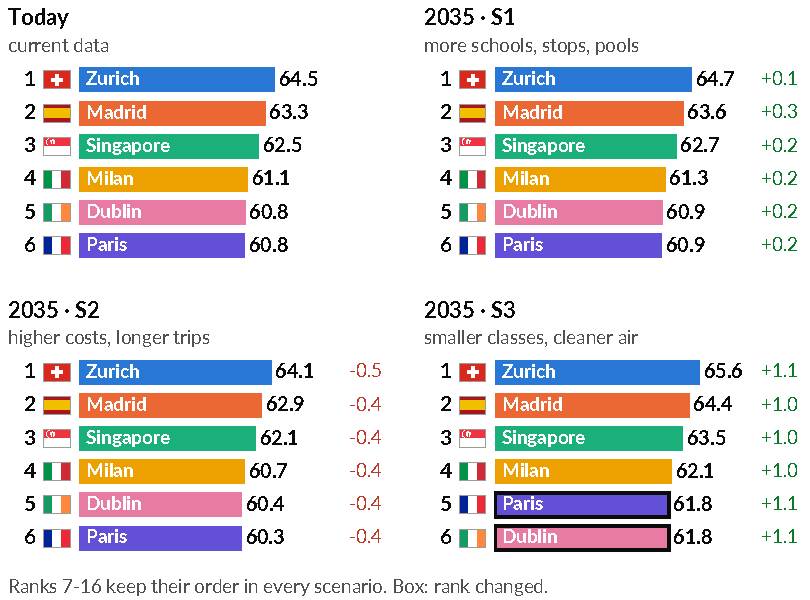
\includegraphics[width=5.4in]{figures/future_2035.pdf}
\caption{Top six cities today and under three hypothetical 2035 scenarios.
Bars show representative scores; numbers give changes from today, and boxes
mark changed ranks. S1: 10\% more higher-education institutions, transit stops
and pools. S2: 10\% higher living costs, housing price-to-income and travel
time. S3: 10\% fewer pupils per teacher, lower PM$_{2.5}$ and shorter travel time.}
\label{fig:future}
\end{figure}

\FloatBarrier
\subsection{Within-city fairness and growth stages}
Citywide supply can mask differences in access and age. Figure~\ref{fig:walktime}
shows walking-time context from resident grids \cite{brunogrids}. Istanbul's 2012
cohort (ages 14--18) has a minimum travel-utility gap of 0.227 between all students
and the lowest fifth \cite{istanbul}. In Oslo's 2023 survey, 66\% of grade 8 and
41\% of final-year upper-secondary respondents rated youth meeting places
positively \cite{osloyouth2023}.

\begin{figure}[!htbp]\centering
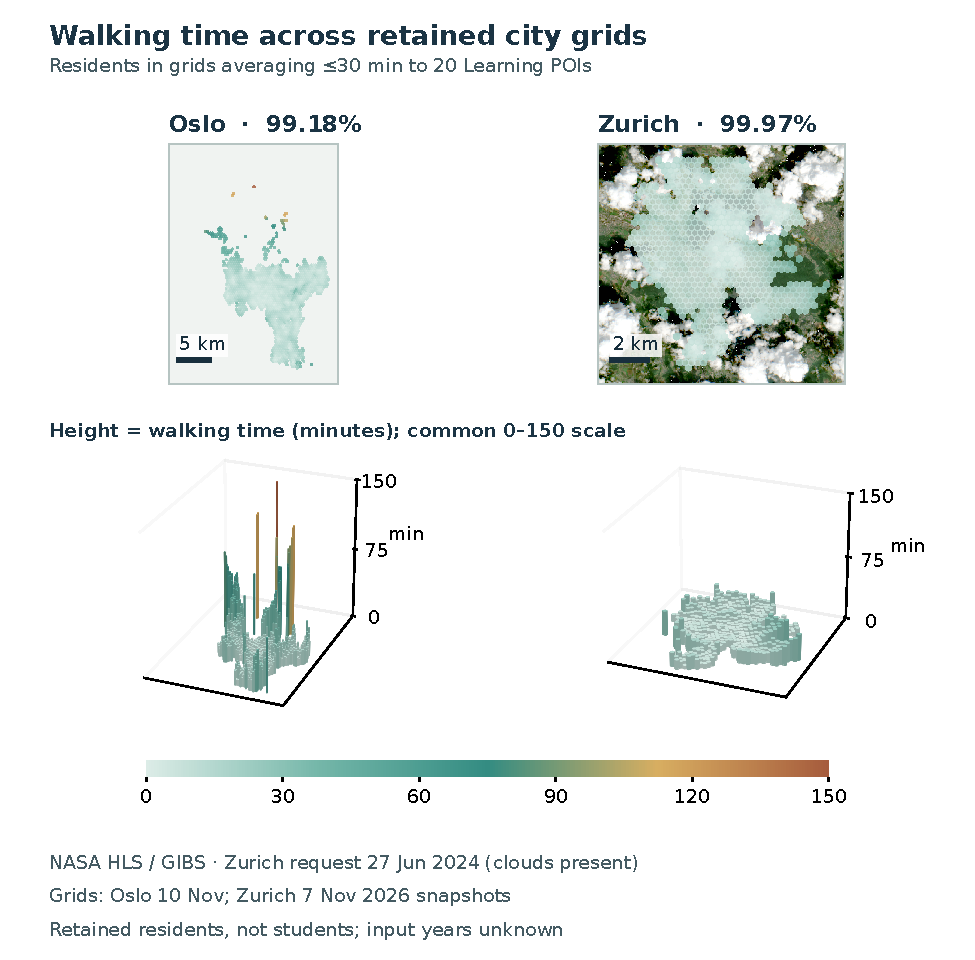
\includegraphics[width=\linewidth]{figures/walktime_context.pdf}
\caption{Walking-time context from the brunogrids resident grids. The modelled mean walking time is measured from resident grid cells to 20 learning POIs, with one common 0--150 minute scale. Among retained residents, 99.18\% of Oslo and 99.97\% of Zurich fall within 30 minutes. This context uses the source's resident grids and is not part of the ten-indicator score.}\label{fig:walktime}
\end{figure}

\FloatBarrier
\section{Conclusion and decision use}
Zurich is our choice among these sixteen cities under the team's high-schooler
priorities, supported by strong safety and education scores. It leads under AHP
and equal weights, in all 31 source-variant checks, and in 82.8\% of 10,000 weight
trials at $\kappa=100$, with the smallest maximum regret of 6.1 points.
Madrid is 1.2 points behind and leads when Zurich's homicide value is withdrawn
(treated as unknown, utility range $[0,1]$). Broad withdrawals of dated or flagged
entries can also make Madrid or Milan first (Table~\ref{tab:vintage}). All three
hypothetical 2035 scenarios retain Zurich, Madrid and Singapore as the top three.
Families can use this shortlist, then check school options, admission, fees and
daily routes against the student's needs.

\clearpage
\phantomsection\addcontentsline{toc}{section}{News article}\label{news-start}
\section*{A city choice built around a student's day}
Zurich is our first choice among sixteen cities for a high schooler, with
64.5 points. Madrid follows just 1.2 points behind, and Singapore takes third.
The result gives families a starting point for comparing places to live and study.

\subsection*{What matters during a school day?}
We scored each city on ten everyday measures and weighted them by what matters
most to a teenager. These cover safety, air quality, living and housing costs,
teaching resources, higher education, transport stops, travel time, broadband
and swimming facilities. Our team chose the priorities, giving safety and
education the greatest influence.

Zurich combines strong school resources and safety with transport and daily
facilities that help balance its higher costs. It stays first in all 31 comparisons
using different counting rules and sources for stops, pools and travel. Treating
all 64 entries dated after 2025 as unknown puts Madrid first; doing so for 28
entries flagged for data concerns, or all 95 entries in the combined date-and-quality
check, puts Milan first. Zurich leads in 82.8\% of 10,000 alternative priority
choices clustered around our team's priorities. When uncertain evidence works
against each city, Zurich falls fewer points behind the best rival than any other choice.

\subsection*{Why Madrid deserves a close look}
Zurich's lead depends on its homicide figure. We use 0.45 per 100,000, calculated
from two completed homicide offences recorded by the Zurich city police in 2025
and 440,935 residents \cite{zhpks2025}. A rate based on two events is unstable.
Zurich stays first up to about 0.69 per 100,000, about three offences a year.
Treating its homicide figure as unknown puts Madrid first.

Eleven entries use substitutes: six national pupil-teacher ratios from Eurostat,
two median ratios for Zurich and London, and three survey travel means. The travel means
allow a span of possible scores. Zurich's homicide recalculation is separate
from these substitutes.

\subsection*{Making the choice personal}
Families should check school admission, language, friendships and wellbeing
alongside the scores. A stop count needs a suitable route and timetable; a
pool count needs affordable fees and usable opening hours. Visiting schools
and trying the daily journey can help settle a close choice.

Zurich remains first when we double the importance of schooling or travel
separately. Three possible 2035 scenarios also keep Zurich, Madrid and Singapore
at the top, with Dublin and Paris switching places in one scenario. These tests
show how the scores respond to changes in services, costs, schools and air quality.
\label{news-end}
\clearpage
\phantomsection\addcontentsline{toc}{section}{References}
\begin{thebibliography}{99}
\raggedright\scriptsize
\setlength{\parskip}{0pt}\setlength{\itemsep}{-1pt}\setlength{\parsep}{0pt}\interlinepenalty=10000
\bibitem{teamtable} Team-supplied city-indicator table, sixteen cities.
Input table, November 2026; supplied values, years and flags retained.
\bibitem{saaty} T. L. Saaty. The analytic hierarchy process: what it is and
how it is used. \textit{Mathematical Modelling}, 9(3--5), 161--176, 1987.
\url{https://doi.org/10.1016/0270-0255(87)90473-8}.
\bibitem{topsis} C.-L. Hwang and K. Yoon. \textit{Multiple Attribute Decision
Making: Methods and Applications}. Springer, 1981.
\url{https://doi.org/10.1007/978-3-642-48318-9}.
\bibitem{enturstop} Entur. National Stop Place Registry, Oslo export dated 9 November 2026; NeTEx stop-place and parent-group definitions. \url{https://developer.entur.org/pages-nsr-nsr/}; \url{https://enturas.atlassian.net/wiki/plugins/viewsource/viewpagesrc.action?pageId=3846668311}.
\bibitem{prague} Czech Statistical Office. \textit{Schools and school facilities,
2024/25}, Tables 3.1.3 and 6.1.18.
\url{https://csu.gov.cz/docs/107508/299702e7-bc0a-1dc2-87db-600d0303f2f4/23004225.pdf?version=1.1}.
\bibitem{singapore} Singapore Department of Statistics. \textit{Census of
Population 2020, Statistical Release 2}, Tables 93 and 124; official Parliament
mirror and official data API.
\url{https://www.parliament.gov.sg/docs/default-source/default-document-library/cop2020sr2.pdf}.
\bibitem{openai} OpenAI. Codex, AI-assisted research, coding, checking and writing
environment. Used November 2026.
\url{https://openai.com/codex/}.
\bibitem{exa} Exa. \texttt{web\_fetch\_exa}, official-source retrieval and text
extraction. Used November 2026. \url{https://exa.ai/}.
\bibitem{warsaw2022} PBS/TRAKO for the Warsaw Metropolitan Area. \textit{Raport nr 2 z diagnozy zachowa\'n transportowych mieszka\'nc\'ow}, July 2022, pp.~3--4, 58, 64. Fieldwork 12 March--30 April 2022; city school-travel sample base 22. Original retrieved 9 November 2026.
\url{https://omw.um.warszawa.pl/wp-content/uploads/2022/09/Raport-nr-2-glowny.pdf}
\bibitem{cbshomicide2022} Statistics Netherlands (CBS). \textit{Meer mensen vermoord in 2022, meeste slachtoffers in Rotterdam}, 29 August 2023; provisional annual city table, and accompanying \textit{Slachtoffers moord en doodslag 2022}, Table 7, period 2018--2022. Originals retrieved 9 November 2026.
\url{https://www.cbs.nl/item?sc_itemid=209e5ed2-506c-42d6-b414-49d3556810bf}
\url{https://www.cbs.nl/nl-nl/maatwerk/2023/35/slachtoffers-moord-en-doodslag-2022}
\bibitem{zhpks2025} Kantonspolizei Z\"urich. \textit{Polizeiliche Kriminalstatistik Kanton Z\"urich 2025}, pp.~117--118, city totals and definition of a criminal act. Original retrieved 9 November 2026.
\url{https://www.zh.ch/content/dam/zhweb/bilder-dokumente/themen/sicherheit-justiz/delikte-praevention/dokumente/pks/aktuell/jahresbericht_2025.pdf}
\bibitem{eurostatcommute} Eurostat.
\textit{Transport---cities and greater cities}, dataset urb\_ctran,
TT1019V, average time of journey to work (minutes).
Retrieved 10 November 2026: IE001C/2011, 28.8; CH002C/2024, 39.9,
flag e (estimated); NO001C/2009, 31.0. Current labels are Dublin, Zurich and
Oslo (greater city);
exact historical boundary and survey window are not established here.
\url{https://ec.europa.eu/eurostat/databrowser/view/urb_ctran/default/table?lang=en}.
\bibitem{tokyooedo} Tokyo Metropolitan Government, Bureau of Transportation.
\textit{Oedo Line station list, Toei Subway ticket-service directory}.
Original CSV, 38 named stations; catalogue created 1 September and updated
4 September 2026; inventory reference date unstated. Retrieved 9 November 2026 UTC.
CC BY (version unspecified).
\url{https://spec.api.metro.tokyo.lg.jp/spec/t000018d0000000027-2911e010ab42b6f8fad459fc7dc10e83-0?lang=en};
\url{https://www.opendata.metro.tokyo.lg.jp/kotsu/subway/subway_branch_o_stationlist.csv}.
\bibitem{warsawmetro} Metro Warszawskie.
\textit{M1 and M2 route station directories}; retrieved 9 November 2026 UTC.
\url{https://metro.waw.pl/metro-warszawskie/linia-m1/przebieg/};
\url{https://metro.waw.pl/metro-warszawskie/linia-m2/przebieg/}.
\textit{Network plan}, marked April 2024; the hosting path is not its content date.
\url{https://metro.waw.pl/wp-content/uploads/2026/02/PLAN-METRA_2.pdf}.
\bibitem{brunogrids} M. Bruno, H. P. Monteiro Melo, B. Campanelli and V. Loreto.
A universal framework for inclusive 15-minute cities. \textit{Nature Cities},
1, 633--641, 2024. \url{https://doi.org/10.1038/s44284-024-00119-4}.
Author-platform resident grids for Singapore and Zurich, accessed 7 November 2026:
\url{https://whatif.sonycsl.it/15mincity/}.
\bibitem{osloyouth2023} A. Bakken. \textit{Ung i Oslo 2023: Ungdomsskolen og videreg\aa{}ende}, NOVA Rapport 6/23, OsloMet, pp.~1, 27, 33, 79--80. Vg3 is the final upper-secondary year. Survey participants: 14,667 lower-secondary (78\% response) and 10,595 upper-secondary (60\% response).
\url{https://oda.oslomet.no/oda-xmlui/bitstream/handle/11250/3065089/NOVA-Rapport-6-2023.pdf}.

\bibitem{vikor} S. Opricovic and G.-H. Tzeng. Compromise solution by MCDM
methods: A comparative analysis of VIKOR and TOPSIS.
\textit{European Journal of Operational Research}, 156(2), 445--455, 2004.
\url{https://doi.org/10.1016/S0377-2217(03)00020-1}.
\bibitem{oslo} City of Oslo, municipal transport GIS, layer 800; Norwegian
Mapping Authority, municipality 0301 boundary. Accessed November 2026.
\url{https://geodata.bymoslo.no/arcgis/rest/services/geodata/Temadata_Publikum/MapServer/800}.
\bibitem{vbz} Verkehrsbetriebe Z\"urich. \textit{Zahlen und Fakten 2025}, p.~6.
\url{https://www.stadt-zuerich.ch/content/dam/vbz/de/die-vbz/zahlen-fakten/geschaeftsbericht/Z4690_VBZ_FB-2025_Web.pdf}.
\bibitem{helsinki} Metropolitan Area Transport Ltd. \textit{Metrolla}.
Official operator inventory, accessed November 2026.
\url{https://kaupunkiliikenne.fi/liikennointi/metrolla/}.
\bibitem{stockpool} City of Stockholm. \textit{Simhallarna} and current swimming
overview. Accessed 8 November 2026.
\url{https://motionera.stockholm/trana-gymma-simma/simhallarna/}.
\bibitem{apur} Atelier parisien d'urbanisme. \textit{Atlas des activit\'es \`a
Paris}, March 2022, p.~37. Sources RATP 2021 and Apur 2022.
\url{https://www.apur.org/sites/default/files/atlas_activites_paris_immobilier.pdf}.
\bibitem{kolada} RKA/Kolada, indicator N17816, Stockholm municipality 0180,
period 2025; source Skolverket (Siris). Definition and total-provider scope
archived with the API response.
\url{https://api.kolada.se/v3/data/kpi/N17816/municipality/0180/year/2025}.
\bibitem{parisedu} Acad\'emie de Paris. \textit{Chiffres cl\'es 2025},
2024 school-entry pupils and 31 December 2024 teacher totals.
\url{https://www.ac-paris.fr/sites/ac_paris/files/2025-08/chiffres-cl-s-acad-mie-de-paris-44994.pdf}.
\bibitem{dublin} Dublin City Council and National Transport Authority.
\textit{Dublin City Centre Transport Plan 2023, Technical Note 6},
issued 2024, Figure 3-7.
\url{https://www.dublincity.ie/sites/default/files/2024-04/06-dublin-city-centre-transport-plan-public-transport-technical-note.pdf}.

\bibitem{shanghai} Shanghai Municipal Education Commission. Regular secondary-school pupil and teacher tables, school year 2025. \url{https://edu.sh.gov.cn/xxgk2_zhzw_tjsj_01/20260610/890926a33cbf443d9abf07c6f65b7734.html}.
\bibitem{sgage} Singapore Ministry of Education. Secondary enrolment by level and age, 2020. \url{https://data.gov.sg/datasets/d_cc84fc751ef5106d9e26cfdbf61776c8/view}.
\bibitem{istanbul} Istanbul Metropolitan Municipality. 2012 household transport survey, official data-portal response resource \texttt{a75118db-28c9-4fdf-b367-d5933b7bb810}; questionnaire, report and nonidentifying aggregate audit archived.
\bibitem{madridmetro} Consorcio Regional de Transportes de Madrid. M4 Estaciones, register dated 29 May 2026; municipality code and network-station identifiers. Accessed 9 November 2026.
\url{https://services5.arcgis.com/UxADft6QPcvFyDU1/arcgis/rest/services/M4_Red/FeatureServer/0}.
\bibitem{inecodes} Instituto Nacional de Estad\'istica. Transport statistics metadata, municipal classification, 2026.
\url{https://www.ine.es/dynt3/metadatos/RespuestaDatos.html?oper=297}.
\bibitem{nerimapool} Nerima City. Municipal swimming inventory and linked venue pages, accessed 9 November 2026.
\url{https://www.city.nerima.tokyo.jp/shisetsu/koen/index.html}.
\bibitem{nerimaclose} Nerima City. Heiwadai closure, 27 October 2026; Miharadai planned closure, 29 September 2026.
\url{https://www.city.nerima.tokyo.jp/kankomoyoshi/sports/oshirase/20261027.html};
\url{https://www.city.nerima.tokyo.jp/kankomoyoshi/sports/oshirase/20260929.html}.
\bibitem{irelandfte} Department of Education and Youth, Ireland. \textit{Teacher Workforce Data Quality Report}, 2026, Sections 5.2 and 8.4.
\url{https://nationaldata.ie/media/NationalDataie/MethodologyDocumentation/Teacher_Workforce_Data_Quality_Report.pdf}.
\bibitem{viennaogd} Wiener Linien. Versioned operator OGD files and
\textit{Beschreibung der OGD-Dateien}, v1.3 (2022), p.~4. Export version
8 November 2026; accessed 9 November 2026. DIVA areas group stopping
positions. GTFS and passenger timetable catalogue retrieved 11 November 2026;
GTFS service-day subset dated 10 November.
\url{https://www.wienerlinien.at/ogd_realtime/doku/};
\url{https://www.wienerlinien.at/fahrplaene}.
\bibitem{viennagis} City of Vienna. Existing U-Bahn stops and Vienna boundary,
OGD WFS layers \texttt{UBAHNHALTOGD} and \texttt{LANDESGRENZEOGD}.
Accessed 9 November 2026; boundary record dated 1 September 2026.
Datenquelle: Stadt Wien -- data.wien.gv.at.
\url{https://data.wien.gv.at/daten/geo?service=WFS&request=GetCapabilities}.
\bibitem{pidmetro} Prague Integrated Transport (PID). \textit{Zast\'avky v Praze},
Prague-only station lists (9 November 2026), native stop data and GTFS
service dated 10 November 2026; public request-stop policy from June 2024.
\url{https://pid.cz/o-systemu/opendata/};
\url{https://pid.cz/vsechny-zastavky-autobusu-a-trolejbusu-v-ramci-pid-budou-na-znameni/}.
\bibitem{dpp2025} Dopravn\'i podnik hlavn\'iho m\v{e}sta Prahy.
\textit{Annual Report 2025}, PDF pp.~17 and 103. Line appearances and
distinct interchange complexes retained separately.
\url{https://www.dpp.cz/spolecnost/o-spolecnosti/vyrocni-zpravy}.
\bibitem{floraclose} Dopravn\'i podnik hlavn\'iho m\v{e}sta Prahy.
Flora station closure from 2 February 2026 until further notice; Florenc C
partial accessibility restriction. Accessed 9 November 2026.
\url{https://www.dpp.cz/omezeni-a-mimoradne-udalosti/detail/15};
\url{https://www.dpp.cz/omezeni-a-mimoradne-udalosti/detail/39}.
\bibitem{bvg} Berliner Verkehrsbetriebe (BVG). U1--U9 official route profiles and tariff-zone definitions. Native station identifiers, station-level zone A and interchange declarations; accessed 9 November 2026.
\url{https://www.bvg.de/de/verbindungen/linienuebersicht}
\url{https://www.bvg.de/de/abos-und-tickets/tarifzonen-und-tarifbestimmungen}
\bibitem{deppmatch} Minist\`ere de l'\'Education nationale, DEPP. Institution personnel indicators and general/technological lyc\'ee pupil counts, rentr\'ee 2025; Henri-IV UAI 0750654D. Teacher ETP covers the institution, not a published upper-stage allocation. Accessed 9 November 2026.
\url{https://data.education.gouv.fr/explore/dataset/fr-en-indicateurs_personnels_etablissements2d/}
\url{https://data.education.gouv.fr/explore/dataset/fr-en-lycee_gt-effectifs-niveau-sexe-lv/}
\bibitem{deppdirectory} Minist\`ere de l'\'Education nationale. Official school directory, Henri-IV UAI 0750654D, row updated 7 November 2026; post-baccalaureate flag. Accessed 9 November 2026.
\url{https://data.education.gouv.fr/explore/dataset/fr-en-annuaire-education/}
\bibitem{tflinventory} Transport for London. Unified API, tube-mode StopPoint inventory and StopTypes metadata; accessed 9 November 2026. Native station and hub identifiers distinguish station entities from platforms and entrances.
\url{https://api.tfl.gov.uk/StopPoint/Mode/tube}
\url{https://api.tfl.gov.uk/StopPoint/Meta/StopTypes}
\bibitem{onslondon} Office for National Statistics. Regions (December 2025) Boundaries EN BFC, full-resolution coastline-clipped geometry; London region E12000007. Accessed 9 November 2026.
\url{https://services1.arcgis.com/ESMARspQHYMw9BZ9/arcgis/rest/services/Regions_December_2025_Boundaries_EN_BFC/FeatureServer/0}
\bibitem{sgbus_lta} Land Transport Authority, Singapore. Bus Stop Location,
Data.gov.sg catalogue and GeoJSON; retrieved 7 November 2026. Archived original
geometry and catalogue HTML; count uses distinct nonempty native bus-stop codes.
\url{https://data.gov.sg/datasets/d_3f172c6feb3f4f92a2f47d93eed2908a/view}
\bibitem{sgpool_directory} Sport Singapore, ActiveSG Circle. Swimming pool
facility directory and 25 linked venue details, retrieved 10 November 2026.
\url{https://www.activesgcircle.gov.sg/facilities/swimming-pools}.
\bibitem{sgocbc} The Kallang. OCBC Aquatic Centre and swimming information, captured 10 November 2026; inventory date unstated. \url{https://www.thekallang.com.sg/en/plan-your-visit/venues-and-amenities/ocbc-aquatic-centre.html}; \url{https://www.thekallang.com.sg/en/things-to-do/sports/swimming.html}.
\bibitem{sgpool_2025} Sport Singapore, ActiveSG Circle. \textit{Editors' pick:
must-hit pools in Singapore}, published 23 April 2025; retrieved 8 November
2026. Archived provider-extracted text and linked venue details; current
pages corroborate venue identity, not 2025 opening hours.
\url{https://www.activesgcircle.gov.sg/read/editors-pick-must-hit-pools-in-singapore}
\bibitem{warsawedu2025} Statistical Office in Warszawa. \textit{Statistical
Yearbook of Warsaw 2025}, education workbook and PDF pp.~156--160, 165;
rounding note p.~22. School-year 2024/25 tables; archived original workbook.
\url{https://new.stat.gov.pl/en/publications-portal/statistical-yearbook-warsaw-2025}
\bibitem{zurichpool} City of Z\"urich. Municipal indoor and school-pool directory
and linked venue details. Original HTML retrieved 10 November 2026, including
W\"armebad K\"aferberg; public-session and holiday restrictions retained.
\url{https://www.stadt-zuerich.ch/de/stadtleben/sport-und-erholung/sport-und-badeanlagen/hallenbaeder.html}
\bibitem{milanpool2025} Milanosport. Swimming-pool tariffs effective 1 June
2025, updated 9 September 2025. Retrieved 8 November 2026; archived
provider-extracted PDF representation, tariff groups A and B.
\url{https://www.milanosport.it/workspace/uploads/nuovi-tariffari-1-giugno-2025-agg-9-10-2025.pdf}
\bibitem{stockholmmetro2025} City of Stockholm and Local Police Area
V\"allingby. \textit{L\"agesbild 2025}, PDF p.~11 (printed p.~10),
Bromma and H\"asselby-V\"allingby metro stations; retrieved 8 November 2026.
Archived original report.
\begingroup\def\UrlBreaks{\do\/\do-\do\?}\url{https://meetingspublic.stockholm.se/welcome-sv/namnder-styrelser/hasselby-vallingby-stadsdelsnamnd/mote-2025-12-18/agenda/6-lagesbild-2025-samverkansoverenskommelse-mellan-hasselby-vallingby-sdf-och-lokalpolisomrade-vallingbypdf?downloadMode=open}\endgroup
\bibitem{milanmetro} Comune di Milano. Stazioni\_Metro, ATM\_Metro MapServer layer 0; metadata date 16 October 2024. Original station and ID responses retrieved November 2026; municipal code 015146 and five operator-map interchange pairs retained.
\url{https://gisportal.comune.milano.it/server/rest/services/D_Mobilita/ATM_Metro/MapServer/0}.
ATM, metro/suburban network map, V26B label, publication date unreported.
\url{https://www.atm.it/it/AltriServizi/Trasporto/Documents/schema_rete_metro.pdf}.
\bibitem{irelandpayroll} Department of Education and Youth.
\textit{The Teaching Workforce in Ireland: Primary and Post Primary Level,
2025/26 School Year}. April 2026, Table 10, p.~14; November 2025 payroll.
\url{https://assets.gov.ie/static/documents/5935f213/Teacher_Workforce_Data_Report_2026.pdf}.
\bibitem{finlandfte} Statistics Finland / Eurostat. Finland UOE national
reference metadata, Annex III--Additional tables, sheet 15.2.2, cell F10.
National metadata updated 1 October 2026; original workbook retrieved
9 November 2026. Full-time/part-time and FTE estimation methods.
\url{https://ec.europa.eu/eurostat/cache/metadata/Annexes/educ_uoe_enr_esmsed_fi_an_Annex_III_-_Additional_tables.xlsx}.
\bibitem{amsterdammetro2026} Gemeente Amsterdam.
\textit{Tram en metro: haltes}, Maps Amsterdam open geodata,
TRAMMETRO\_PUNTEN\_2026; metadata ID 649, 2026, exact observation date unreported; municipal boundary
INDELING\_GEMEENTE, March 2026.
Original GeoJSON and metadata retrieved 9 November 2026.
\url{https://maps.amsterdam.nl/open_geodata/?k=649}.
\bibitem{cbsboundary2025} Statistics Netherlands (CBS) / PDOK.
\textit{CBS Gebiedsindelingen 2025}, non-generalised municipal boundary,
GM0363 Amsterdam; retrieved 9 November 2026. CC BY 4.0.
\url{https://service.pdok.nl/cbs/gebiedsindelingen/2025/wfs/v1_0?service=WFS&request=GetCapabilities}.
\bibitem{warsawfirescope} Mazovian Provincial Headquarters, State Fire Service.
\textit{Information bulletin for 2025}, published February 2026, physical p.~4.
Locates 21 M1 and 18 M2 station appearances within Warsaw; the shared interchange
is consolidated using the operator directories.
\url{https://www.gov.pl/attachment/2b7775c0-aa52-487e-809a-66df1b991b59}.
\bibitem{numbeooslo2026} Numbeo. \textit{Property Prices Index by City},
annual 2026 and rolling Current. Archived copies; access date recorded as 7 November 2026.
\url{https://www.numbeo.com/property-investment/rankings.jsp?title=2026};
\url{https://www.numbeo.com/property-investment/rankings_current.jsp}.
\end{thebibliography}
\label{main-end}
\clearpage
\section*{Report on Use of AI Tools}
\addcontentsline{toc}{section}{Report on Use of AI Tools (additional pages)}
The team used AI-assisted retrieval, calculation and drafting during 8--14 November 2026. We checked outputs against official source records, saved retrieval receipts, recomputed model results, and compiled and reviewed the rendered manuscript. The tools below record the uses documented in the team report.\cite{openai,exa}

\begin{table}[!htbp]\centering
\caption{Recorded AI-tool use and checks.}
\begingroup\setlength{\tabcolsep}{4.5pt}
\begin{tabular}{@{}p{.16\linewidth}p{.20\linewidth}p{.29\linewidth}p{.29\linewidth}@{}}
\toprule Tool & Who/when (as recorded) & Used for & How we checked it \\ \midrule
OpenAI Codex & Team record, 8--11 and 14 November 2026 & Official-source search and extraction, data-scope checks, Python calculations and audits, LaTeX drafting, wording revisions, and simulated judge reviews of the draft & Compared claims with source records; recomputed calculations; compiled and reviewed the rendered pages \\ \midrule
Anthropic Claude (Claude Code) & 14 November 2026 & Planning the revision after our advisor's feedback, AHP and scenario calculations, all figures, proxy-data searches, and small text edits & Recomputed every reported number from the result files; inspected each figure at print size \\ \midrule
Exa (\texttt{web\_\allowbreak fetch\_\allowbreak exa}) & Team record, 8--9 November 2026 & Retrieval and text extraction from official webpages, PDFs and data interfaces & Saved source URLs and returned text; checked extracted representations against original downloaded records and excluded ambiguous material \\ \midrule
Anti-defensive-writing skill & Applied during manuscript revision & Editorial guidance for concise, evidence-supported wording & Reviewed claims against the manuscript evidence and retained conclusion-changing checks \\ \bottomrule
\end{tabular}\endgroup
\end{table}

Usage by other team members: to be added by the team before submission.

\end{document}
